%
% nichtkomm.tex
%
% (c) 2021 Prof Dr Andreas Müller, OST Ostschweizer Fachhochschule
%
\documentclass[tikz]{standalone}
\usepackage{times}
\usepackage{amsmath}
\usepackage{txfonts}
\usepackage[utf8]{inputenc}
\usepackage{graphics}
\usetikzlibrary{arrows,intersections,math}
\usepackage{ifthen}
\begin{document}

\definecolor{darkgreen}{rgb}{0,0.6,0}

\newboolean{showgrid}
\setboolean{showgrid}{false}
\def\breite{7}
\def\hoehe{4}

\begin{tikzpicture}[>=latex,thick]

% Povray Bild
\node at (0,0) {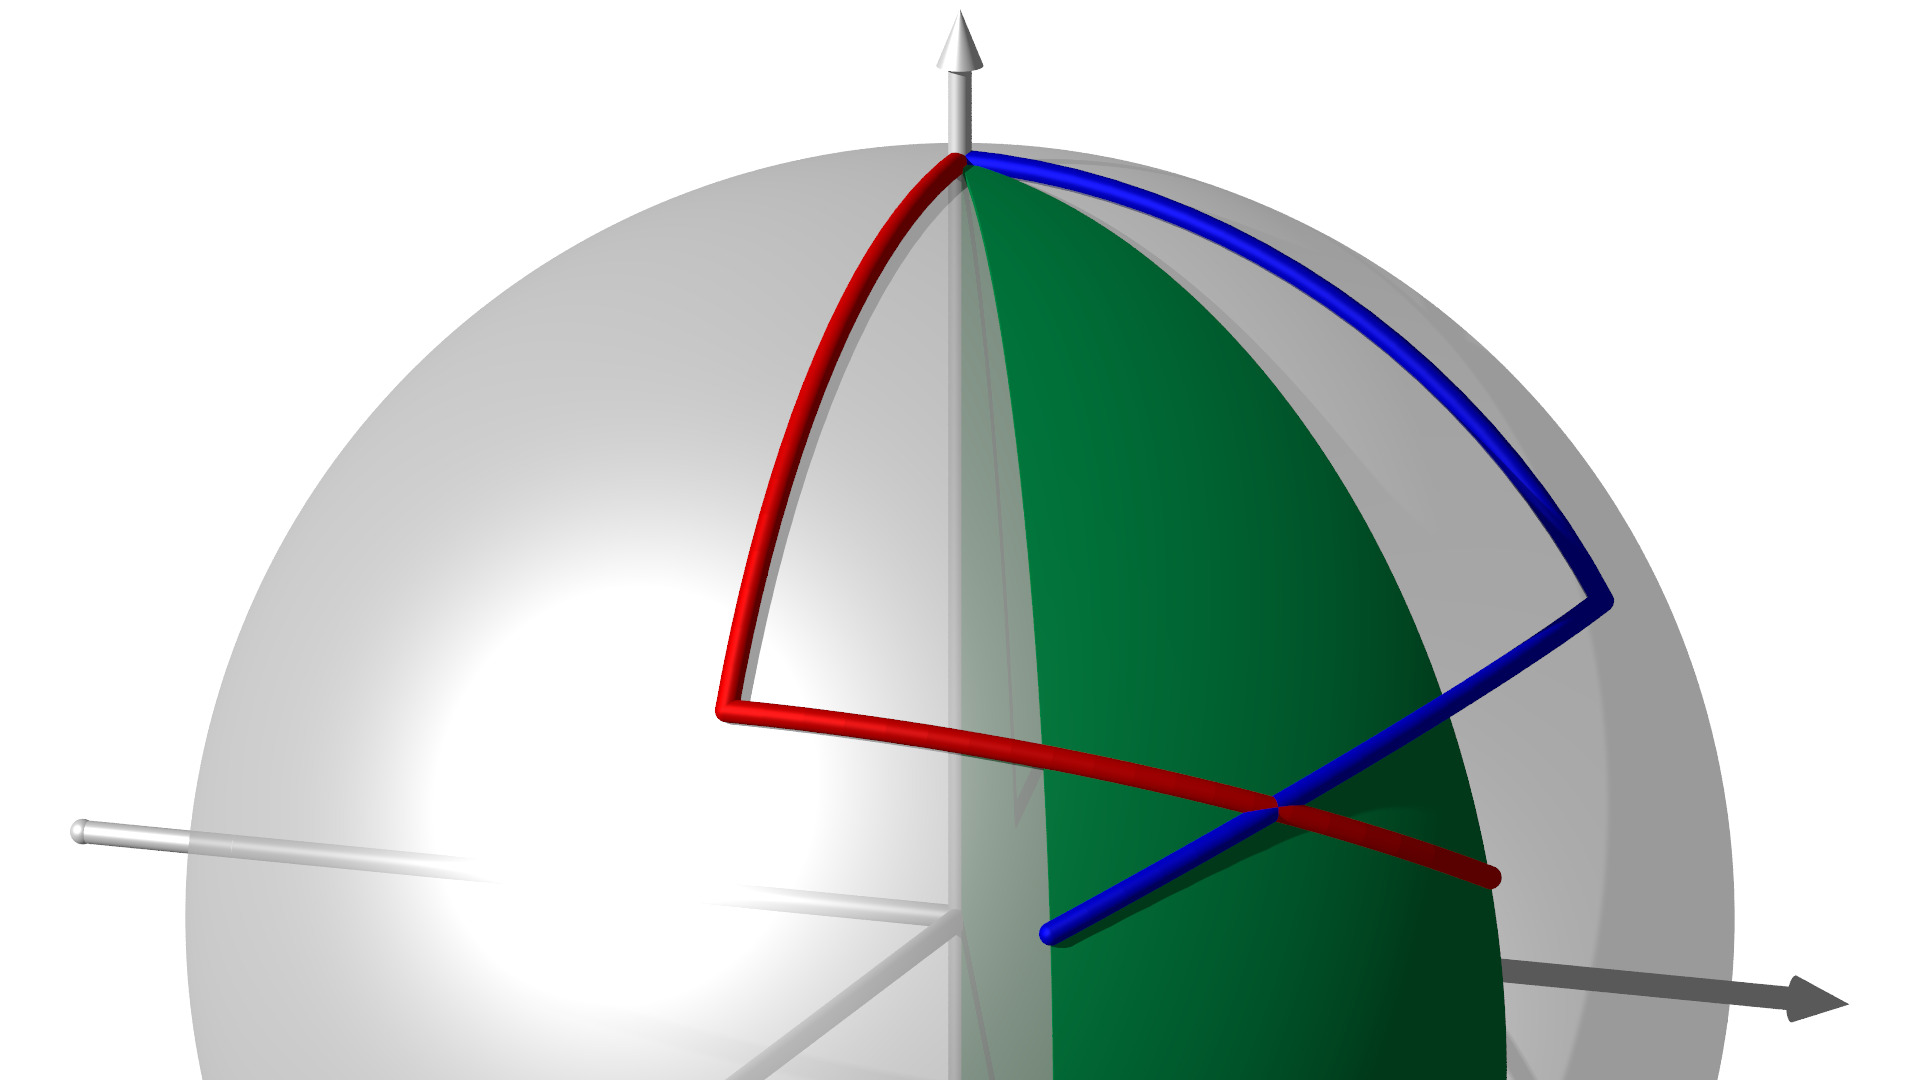
\includegraphics[width=14cm]{c60.jpg}};

% Gitter
\ifthenelse{\boolean{showgrid}}{
\draw[step=0.1,line width=0.1pt] (-\breite,-\hoehe) grid (\breite, \hoehe);
\draw[step=0.5,line width=0.4pt] (-\breite,-\hoehe) grid (\breite, \hoehe);
\draw                            (-\breite,-\hoehe) grid (\breite, \hoehe);
\fill (0,0) circle[radius=0.05];
}{}

\coordinate (A) at (-0.3,3);
\coordinate (B) at (-1.1,2);
\coordinate (C) at (-2.1,-1.2);
\draw[->,color=red,line width=1.4pt]
        (A)
        to[out=-143,in=60]
        (B)
        to[out=-120,in=80]
        (C);
%\fill[color=red] (B) circle[radius=0.08];
\node[color=red] at (-1.2,1.5) [above left] {$R_{x_1,\alpha}$};
\coordinate (D) at (0.3,3.2);
\coordinate (E) at (1.8,2.8);
\coordinate (F) at (5.2,-0.3);
\draw[->,color=blue,line width=1.4pt]
        (D)
        to[out=-10,in=157]
        (E)
        to[out=-23,in=120]
        (F);
%\fill[color=blue] (E) circle[radius=0.08];
\node[color=blue] at (2.4,2.4) [above right] {$R_{x_2,\beta}$};
\draw[->,color=darkgreen,line width=1.4pt]
        (0.7,-3.1) to[out=1,in=-160] (3.9,-2.6);
\node[color=darkgreen] at (2.5,-3.4) {$R_{x_3,\gamma}$};

\node at (6.4,-2.9) {$x_1$};
\node at (-0.2,3.8) {$x_3$};

\end{tikzpicture}

\end{document}

